%%%%%%%%%%%%%%%%%%%%%%%%%%%%%%%%%%%%%%%%%%%%%%%
%%% SECTION 1: ROOFLINE
%%%%%%%%%%%%%%%%%%%%%%%%%%%%%%%%%%%%%%%%%%%%%%%
\section{Roofline}

%%%%%%%%%%%%%%%%%%%%%%%%%%%%%%%%%%%%%%%%%%%%%%%
%%% SUBECTION 1.1: Profiling
%%%%%%%%%%%%%%%%%%%%%%%%%%%%%%%%%%%%%%%%%%%%%%%
\subsection{Profiling}
The computer characterized here is the HP dv5-1170ep, released in 2008.

Most of the hardware was obtained from the Intel ARK Website \cite{ark} and from standard Linux tools:
\begin{description}
\item[dmidecode] Tool for hardware dump from BIOS information;
\item[lscpu] Lists CPU information;
\item[lshw] Lists hardware information
\item[getconf] Lists various configuration variables (e.g. cache organization values)
\end{description}

AIDA64 Extreme Edition for Windows 7 was used to measure memory latencies (\autoref{fig:aida64}). It's results were then compared against the previosly obtained data to ensure it's accuracy.
Some of the data is theorethically calculated based on the given hardware characteristics. This, of course, represents only a theorethical limit for the hardware, and not actually measured data.

%%%%%%%%%%%%%%%%%%%%%%%%%%%%%%%%%%%%%%%%%%%%%%%
%%% SUBSUBSECTION 1.1.1: Peak FP Performance
%%%%%%%%%%%%%%%%%%%%%%%%%%%%%%%%%%%%%%%%%%%%%%%
\subsubsection{Peak Floating-Point Performance}
In order to keep coherency with the Roofline paper\cite{roofline}, Peak FP Performance was measured using double-precision floating point numbers. The formula to calculate the maximum double precision floating point throughput is:

$$\mathrm{Flop/s_{max}} = T_{\mathrm{FP}} \times f_{\mathrm{clock}} \times \#_{\mathrm{cores}}$$

Where $T_{\mathrm{FP}}$ is the double precision floating point throughput of each core.

The CPU in question, Core 2 Duo P8600, has two cores working with a clock rate of 2.4 GHz. Being based on the Core micro architecture, each core has one execution unit for 128-bit floating point addition, and one for multiplication. When considering SIMD operations, with the SSE and MMX extensions, then each 128-bit register can carry two double precision floating point values, thus effectively doubling the throughput. With an ideal multiply/add balance, four floating point operations can run in parallel.

\begin{IEEEeqnarray}{CrClC}
\Rightarrow		& \mathrm{Flop/s_{max}} & = & 4 \times \left (2.4 \times 10^9 \right ) \times 2 & \Leftrightarrow	\nonumber \\
\Leftrightarrow	& \mathrm{Flop/s_{max}} & = & 19.2\;\mathrm{GFlop/s} & \nonumber
\end{IEEEeqnarray}

%%%%%%%%%%%%%%%%%%%%%%%%%%%%%%%%%%%%%%%%%%%%%%%
%%% SUBSUBSECTION 1.1.2: Peak Mem BW
%%%%%%%%%%%%%%%%%%%%%%%%%%%%%%%%%%%%%%%%%%%%%%%
\subsubsection{Peak Memory Bandwidth}
This value can be calculated based on the memory clock rate and the memory bus. Multiple channels should also be taken into account.
The memory is a SDRAM DDR2 operating at a clock rate of 800MHz, and using two modules, taking advantage of the dual-channel. The bus width is 64 bits (or 8 Bytes)

\begin{IEEEeqnarray}{CrClC}
\Rightarrow		& \mathrm{BW_{max}} & = & MEM_{\mathrm{clock}} \times bus_{\mathrm{width}} \times \#\mathrm{channels} & \Leftrightarrow \\
\Leftrightarrow	& \mathrm{BW_{max}} & = & (800 \times 10^9) \times 64 \times 2 & \Leftrightarrow \nonumber \\
\Leftrightarrow & \mathrm{BW_{max}} & = & 12.8\;\mathrm{GB/s} & \nonumber
\end{IEEEeqnarray}


%%%%%%%%%%%%%%%%%%%%%%%%%%%%%%%%%%%%%%%%%%%%%%%
%%% SUBsubSECTION 1.2.3: Summary
%%%%%%%%%%%%%%%%%%%%%%%%%%%%%%%%%%%%%%%%%%%%%%%
\subsubsection{Summary}
The full characterization of the laptop is summarized in \autoref{tab:profile}

\begin{table}[!htp]

\begin{minipage}[t]{0.5\linewidth}
	\vspace{0pt}
	%\begin{center}
		\begin{tabular}{|rl|}
			\multicolumn{2}{c}{\textbf{Laptop}}				\\
			\hline
				Manufacturer		&	HP					\\
				Model				&	Pavilion dv5 1170ep	\\
			\hline
			\multicolumn{2}{c}{} 							\\
			\multicolumn{2}{c}{\textbf{Processor}} 			\\
			\hline
				Manufacturer:		&	Intel				\\
				Model:				&	P8600				\\
				$\mu$-arch			&	Core				\\
				Codename			&	Penryn-3M			\\
				Clock frequency		&	2.4 GHz				\\
				Cores				&	2					\\
				Threads:			&	2					\\
				Peak Flop/s			&	19.2 GFlop/s		\\
			\hline
		\end{tabular}
	%%\end{center}

\end{minipage}
\begin{minipage}[t]{0.5\linewidth}
	\vspace{0pt}
	%\begin{center}

		\begin{tabular}{|c|rl|}
			\multicolumn{3}{c}{\textbf{Memory}}		\\
			\hline
			\multicolumn{1}{|c|}{\multirow{5}{*}{L1}}
				&	Scope			&	Core		\\
				&	Size			&	32KB + 32KB	\\
				&	Associativity	&	8-way		\\
				&	Line Size		&	64 B		\\
				&	Write Policy	&	Write-back	\\
			\hline
			\multicolumn{1}{|c|}{\multirow{5}{*}{L2}}
				&	Scope			&	shared		\\
				&	Size			&	3MB			\\
				&	Associativity	&	12-way		\\
				&	Line Size		&	64 B		\\
				&	Write Policy	&	Write-back	\\
			\hline

			%\textbf{Main Memory:}	&				&					\\
			\multicolumn{1}{|c|}{\multirow{6}{*}{RAM}}
				&	Type			&	SDRAM DDR2 PC6400				\\
				&	Frequency		&	800 MHz							\\
				&	Num. Channels	&	2								\\
				&	Size			&	4 GB							\\
				&	Latency			&	81.1 ns							\\
				&	Peak Bandwith	&	12.8 GB/s						\\
			\hline			
		\end{tabular}
	%\end{center}
\end{minipage}
	\caption{Laptop characterization \label{tab:profile}}
\end{table}
~

\begin{figure}[!htp]
	\begin{center}
		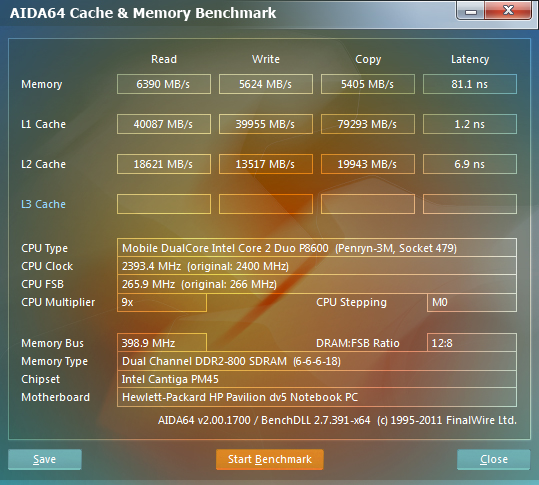
\includegraphics[width=12cm]{images/aida64.png}
		\caption[Memory benchmark]{Memory benchmark with Aida64 Extreme Edition \label{fig:aida64}}
	\end{center}
\end{figure}

%%%%%%%%%%%%%%%%%%%%%%%%%%%%%%%%%%%%%%%%%%%%%%%
%%% SSUBSECTION 2. ROOFLINE MODEL
%%%%%%%%%%%%%%%%%%%%%%%%%%%%%%%%%%%%%%%%%%%%%%%
\subsection{Roofline}

%%%%%%%%%%%%%%%%%%%%%%%%%%%%%%%%%%%%%%%%%%%%%%%
%%% SUSUBSBECTION 2.1. ROOFS
%%%%%%%%%%%%%%%%%%%%%%%%%%%%%%%%%%%%%%%%%%%%%%%
\subsubsection{Roofs}

Based on the data gathered from the laptop characterization, and the information from the Roofline paper \cite{roofline}, both roofs for the model can be easily calculated by the formula:

$$ Flops/sec = min(Peak Flops/sec, Memory Bandwidth \times Op. Intensity ) $$

The first part of the $\mathrm{min}$ function gives the CPU roof, which is equal to the CPU's peak Flop performance. The memory roof increases linearly with the Operational Intensity (as the operational intensity increases, problems become more CPU-bound and less memory-bound)

%%%%%%%%%%%%%%%%%%%%%%%%%%%%%%%%%%%%%%%%%%%%%%%
%%% SUBSUBSECTION 2.2. CEILINGS
%%%%%%%%%%%%%%%%%%%%%%%%%%%%%%%%%%%%%%%%%%%%%%%
\subsubsection{Ceilings}

Ceilings were added to the model by gradually recalculating the roofs without a certain architecture characteristic. Each ceiling is given by the value of the previous ceiling (with the roof being the base value), divided by a factor which represents the weight that the removed characteristic had in the performance. The ceilings estimated were:
\begin{description}
	\item[All cores used]This corresponds to the roof, where all the resources are considered.
	\item[Mul/Add balance, No TLP (only one core)]This ceiling considers only the usage of a single core, against two cores in the previous. This represents a reduction in peak performance by a factor of 2, so the ceiling has half the value of the previous one.
	\item[With SIMD (no Mul/Add balance)]Here, it was considered that multiplication and addition instructions were not balanced. Without this balance, the hardware won't be used to it's full potential. Each core has two SSE units, one unit to process multiplications and another for additions. It also has two normal units, but they can't be used at the same time. So if only one of those is busy at each instant, the performance is again halved.
	\item[ILP Only (no SIMD)]Finally SIMD were removed. Since everything was measured using double-precision floating point numbers, SIMD would allow two FP operations to be processed each clock cycle. Without SIMD, only one will be processed, which is half of the original performance
\end{description}

For the memory, only one ceiling was estimated. This ceiling occurs when dual channel is removed, which theoretically drops memory bandwith to half its value.

\autoref{tab:ceilings} shows a summary of all the ceilings calculated, and it's value

%%%%%%%%%%%%%%%%%%%%%%%%%%%%%%%%%%%%%%%%%%%%%
% TABLE 
\begin{table}[!htp]
	\begin{center}
		\begin{tabular}{c|c|c|}
				&	Ceiling		&	Value (GFlops)				\\
				\hline
				\hline
			\multicolumn{1}{c|}{\multirow{4}{*}{CPU}}
				&	All cores used		&	19.2				\\
				&	Mul/Add balance		&	9.6					\\
				&	With SIMD			&	4.8					\\
				&	ILP Only			&	2.4					\\
			\hline
			\hline
			\multicolumn{1}{c|}{\multirow{2}{*}{Memory}}
				&	All channels used	&	12.8\footnotemark	\\
				&	No dual channel		&	6.4					\\
				\hline
		\end{tabular}
	\end{center}
	\caption{Ceiling values for Roofline Mode \label{tab:ceilings}}
\end{table}
\footnotetext{This value correspondes to an operational intensity of 1}

\autoref{fig:roofline} shows the graph for the Roofline model. \autoref{fig:rooflinex4} shows the same Roofline model overlaped with the Roofline for the Opteron X4, for comparison.

\newpage

\begin{figure}[!htp]
	\begin{minipage}[t]{0.5\linewidth}
		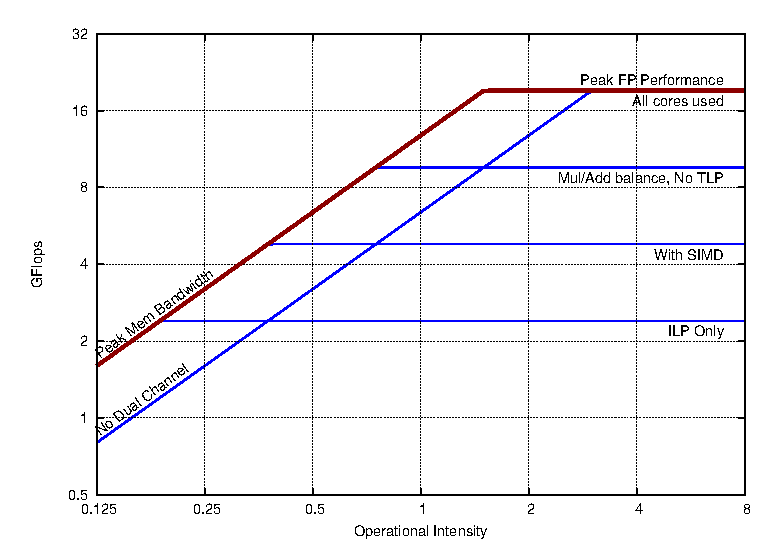
\includegraphics[width=\textwidth]{images/roofline.eps}
		\caption[Roofline Model]{Roofline Model based on laptop characterization \label{fig:roofline}}
	\end{minipage}
	\hspace{0.5cm}
	\begin{minipage}[t]{0.5\linewidth}
		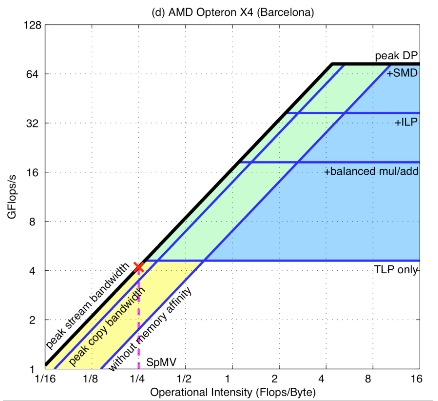
\includegraphics[width=\textwidth]{images/roofline_x4.jpg}
		\caption[Roofline Model with Opteron X4]{Roofline Model based, overlaped with Roofline Model for the Opteron X4 \label{fig:rooflinex4}}
	\end{minipage}
\end{figure}

The main difference between the P8600 used in this article and the Opteron X4 is in the number of cores. Both processors have two SSE units, and two regular units (sharing the issue port with the SSE units) per core, with each SSE isntructions usign 128 bit registers in both processors. So each one can process 2 double precision floating points per cycle(assumind a fully pipelined architecture with a latency of one cycle per instruction). The clock frequency is roughly the same (2.4 GHz in the P8600, 2.3 GHz in the Opteron X4). The Opteron system showed here uses a dual-socket architecture, with two Opteron X4, for a total of 8 cores, four times more than the laptop architecture. This matches the expected values for the roofline model, which shows that the peak performance for the dual Opteron X4 system is around 4 times higher than the laptop.
